\documentclass{ximera}


\graphicspath{
  {./}
  {1-1QuantitativeReasoning/}
  {1-2RelationsAndGraphs/}
  {1-3ChangingInTandem/}
  {2-1LinearEquations/}
  {2-2LinearModeling/}
  {2-3ExponentialModeling/}
  {3-1WhatIsAFunction/}
  {3-2FunctionProperties/}
  {3-3AverageRatesOfChange/}
  {4-1BuildingNewFunctions/}
  {4-2Polynomials/}
  {5-1RationalFunctions/}
   {5-2ExponentialFunctions/}
  {6-1Domain/}
  {6-2Range/}
  {6-3CompositionOfFunctions/}
  {7-1ZerosOfFunctions/}
  {7-XZerosOfPolynomials/}
  {7-2ZerosOfFamousFunctions/}
  {8-0Review/}
  {8-1FunctionTransformations/}
  {8-2SolvingInequalities/}
  {8-3FunctionTransformationsProject/}
  {9-1RightTriangleTrig/}
  {9-2TheUnitCircle/}
  {9-3TrigIdentities/}
  {10-1UnitCircleToFunctionGraph/}
  {10-2TrigFunctions/}
  {10-3SomeApplicationsOfTrig/}
  {11-1InverseFunctionsRevisited/}
  {11-2Logarithms/}
  {11-3InverseTrig/}
  {12-1SystemsOfEquations/}
  {12-2NonlinearSystems/}
  {12-3ApplicationsOfSystems/}
  {13-1SecantLinesRevisited/}
  {13-2Functions-TheBigPicture/}
  {14-1DisplacementVsDistance/}
  {1-1QuantitativeReasoning/exercises/}
  {1-2RelationsAndGraphs/exercises/}
  {../1-3ChangingInTandem/exercises/}
  {../2-1LinearEquations/exercises/}
  {../2-2LinearModeling/exercises/}
  {../2-3ExponentialModeling/exercises/}
  {../3-1WhatIsAFunction/exercises/}
  {../3-2FunctionProperties/exercises/}
  {../3-3AverageRatesOfChange/exercises/}
  {../5-2ExponentialFunctions/exercises/}
  {../4-1BuildingNewFunctions/exercises/}
  {../4-2Polynomials/exercises/}
  {../5-1RationalFunctions/exercises/}
  {../6-1Domain/exercises/}
  {../6-2Range/exercises/}
  {../6-3CompositionOfFunctions/exercises/}
  {../7-1ZerosOfFunctions/exercises/}
  {../7-XZerosOfPolynomials/exercises/}
  {../7-2ZerosOfFamousFunctions/exercises/}
  {../8-1FunctionTransformations/exercises/}
  {../12-1SystemsOfEquations/exercises/}
  {../8-3FunctionTransformationsProject/exercises/}
  {../8-0Review/exercises/}
  {../8-2SolvingInequalities/exercises/}
  {../8-3FunctionTransformationsProject/exercises/}
  {../9-1RightTriangleTrig/exercises/}
  {../9-2TheUnitCircle/exercises/}
  {../9-3TrigIdentities/exercises/}
  {../10-1UnitCircleToFunctionGraph/exercises/}
  {../10-2TrigFunctions/exercises/}
  {../10-3SomeApplicationsOfTrig/exercises/}
  {../11-1InverseFunctionsRevisited/exercises/}
  {../11-2Logarithms/exercises/}
  {../11-3InverseTrig/exercises/}
  {../12-1SystemsOfEquations/exercises/}
  {../12-2NonlinearSystems/exercises/}
  {../12-3ApplicationsOfSystems/exercises/}
  {../13-1SecantLinesRevisited/exercises/}
  {../13-2Functions-TheBigPicture/exercises/}
  {../14-1DisplacementVsDistance/exercises/}
}

\DeclareGraphicsExtensions{.pdf,.png,.jpg,.eps}

\newcommand{\mooculus}{\textsf{\textbf{MOOC}\textnormal{\textsf{ULUS}}}}

\usepackage[makeroom]{cancel} %% for strike outs

\ifxake
\else
\usepackage[most]{tcolorbox}
\fi


%\typeout{************************************************}
%\typeout{New Environments}
%\typeout{************************************************}

%% to fix for web can be removed when deployed offically with ximera2
\let\image\relax\let\endimage\relax
\NewEnviron{image}{% 
  \begin{center}\BODY\end{center}% center
}



\NewEnviron{folder}{
      \addcontentsline{toc}{section}{\textbf{\BODY}}
}

\ifxake
\let\summary\relax
\let\endsummary\relax
\newtheorem*{summary}{Summary}
\newtheorem*{callout}{Callout}
\newtheorem*{overview}{Overview}
\newtheorem*{objectives}{Objectives}
\newtheorem*{motivatingQuestions}{Motivating Questions}
\newtheorem*{MM}{Metacognitive Moment}
      
%% NEEDED FOR XIMERA 2
%\ximerizedEnvironment{summary}
%\ximerizedEnvironment{callout}
%\ximerizedEnvironment{overview} 
%\ximerizedEnvironment{objectives}
%\ximerizedEnvironment{motivatingQuestions}
%\ximerizedEnvironment{MM}
\else
%% CALLOUT
\NewEnviron{callout}{
  \begin{tcolorbox}[colback=blue!5, breakable,pad at break*=1mm]
      \BODY
  \end{tcolorbox}
}
%% MOTIVATING QUESTIONS
\NewEnviron{motivatingQuestions}{
  \begin{tcolorbox}[ breakable,pad at break*=1mm]
    \textbf{\Large Motivating Questions}\hfill
    %\begin{itemize}[label=\textbullet]
      \BODY
    %\end{itemize}
  \end{tcolorbox}
}
%% OBJECTIVES
\NewEnviron{objectives}{  
    \vspace{.5in}
      %\begin{tcolorbox}[colback=orange!5, breakable,pad at break*=1mm]
    \textbf{\Large Learning Objectives}
    \begin{itemize}[label=\textbullet]
      \BODY
    \end{itemize}
    %\end{tcolorbox}
}
%% DEFINITION
\let\definition\relax
\let\enddefinition\relax
\NewEnviron{definition}{
  \begin{tcolorbox}[ breakable,pad at break*=1mm]
    \noindent\textbf{Definition}~
      \BODY
  \end{tcolorbox}
}
%% OVERVIEW
\let\overview\relax
\let\overview\relax
\NewEnviron{overview}{
  \begin{tcolorbox}[ breakable,pad at break*=1mm]
    \textbf{\Large Overview}
    %\begin{itemize}[label=\textbullet] %% breaks Xake
      \BODY
    %\end{itemize}
  \end{tcolorbox}
}
%% SUMMARY
\let\summary\relax
\let\endsummary\relax
\NewEnviron{summary}{
  \begin{tcolorbox}[ breakable,pad at break*=1mm]
    \textbf{\Large Summary}
    %\begin{itemize}[label=\textbullet] %% breaks Xake
      \BODY
    %\end{itemize}
  \end{tcolorbox}
}
%% REMARK
\let\remark\relax
\let\endremark\relax
\NewEnviron{remark}{
  \begin{tcolorbox}[colback=green!5, breakable,pad at break*=1mm]
    \noindent\textbf{Remark}~
      \BODY
  \end{tcolorbox}
}
%% EXPLANATION
\let\explanation\relax
\let\endexplanation\relax
\NewEnviron{explanation}{
    \normalfont
    \noindent\textbf{Explanation}~
      \BODY
}
%% EXPLORATION
\let\exploration\relax
\let\endexploration\relax
\NewEnviron{exploration}{
  \begin{tcolorbox}[colback=yellow!10, breakable,pad at break*=1mm]
    \noindent\textbf{Exploration}~
      \BODY
  \end{tcolorbox}
}
%% METACOGNITIVE MOMENTS
\let\MM\relax
\let\endMM\relax
\NewEnviron{MM}{
  \begin{tcolorbox}[colback=pink!15, breakable,pad at break*=1mm]
    \noindent\textbf{Metacognitive Moment}~
      \BODY
  \end{tcolorbox}
}


\fi





%Notes on what envirnoment to use:  Example with Explanation in text; if they are supposed to answer- Problem; no answer - Exploration


%\typeout{************************************************}
%% Header and footers
%\typeout{************************************************}

\newcommand{\licenseAcknowledgement}{Licensed under Creative Commons 4.0}
\newcommand{\licenseAPC}{\renewcommand{\licenseAcknowledgement}{\textbf{Acknowledgements:} Active Prelude to Calculus (https://activecalculus.org/prelude) }}
\newcommand{\licenseSZ}{\renewcommand{\licenseAcknowledgement}{\textbf{Acknowledgements:} Stitz Zeager Open Source Mathematics (https://www.stitz-zeager.com/) }}
\newcommand{\licenseAPCSZ}{\renewcommand{\licenseAcknowledgement}{\textbf{Acknowledgements:} Active Prelude to Calculus (https://activecalculus.org/prelude) and Stitz Zeager Open Source Mathematics (https://www.stitz-zeager.com/) }}
\newcommand{\licenseORCCA}{\renewcommand{\licenseAcknowledgement}{\textbf{Acknowledgements:}Original source material, products with readable and accessible
math content, and other information freely available at pcc.edu/orcca.}}
\newcommand{\licenseY}{\renewcommand{\licenseAcknowledgement}{\textbf{Acknowledgements:} Yoshiwara Books (https://yoshiwarabooks.org/)}}
\newcommand{\licenseOS}{\renewcommand{\licenseAcknowledgement}{\textbf{Acknowledgements:} OpenStax College Algebra (https://openstax.org/details/books/college-algebra)}}
\newcommand{\licenseAPCSZCSCC}{\renewcommand{\licenseAcknowledgement}{\textbf{Acknowledgements:} Active Prelude to Calculus (https://activecalculus.org/prelude), Stitz Zeager Open Source Mathematics (https://www.stitz-zeager.com/), CSCC PreCalculus and Calculus texts (https://ximera.osu.edu/csccmathematics)}}

\ifxake\else %% do nothing on the website
\usepackage{fancyhdr}
\pagestyle{fancy}
\fancyhf{}
\fancyhead[R]{\sectionmark}
\fancyfoot[L]{\thepage}
\fancyfoot[C]{\licenseAcknowledgement}
\renewcommand{\headrulewidth}{0pt}
\renewcommand{\footrulewidth}{0pt}
\fi

%%%%%%%%%%%%%%%%



%\typeout{************************************************}
%\typeout{Table of Contents}
%\typeout{************************************************}


%% Edit this to change the font style
\newcommand{\sectionHeadStyle}{\sffamily\bfseries}


\makeatletter

%% part uses arabic numerals
\renewcommand*\thepart{\arabic{part}}


\ifxake\else
\renewcommand\chapterstyle{%
  \def\maketitle{%
    \addtocounter{titlenumber}{1}%
    \pagestyle{fancy}
    \phantomsection
    \addcontentsline{toc}{section}{\textbf{\thepart.\thetitlenumber\hspace{1em}\@title}}%
                    {\flushleft\small\sectionHeadStyle\@pretitle\par\vspace{-1.5em}}%
                    {\flushleft\LARGE\sectionHeadStyle\thepart.\thetitlenumber\hspace{1em}\@title \par }%
                    {\setcounter{problem}{0}\setcounter{sectiontitlenumber}{0}}%
                    \par}}





\renewcommand\sectionstyle{%
  \def\maketitle{%
    \addtocounter{sectiontitlenumber}{1}
    \pagestyle{fancy}
    \phantomsection
    \addcontentsline{toc}{subsection}{\thepart.\thetitlenumber.\thesectiontitlenumber\hspace{1em}\@title}%
    {\flushleft\small\sectionHeadStyle\@pretitle\par\vspace{-1.5em}}%
    {\flushleft\Large\sectionHeadStyle\thepart.\thetitlenumber.\thesectiontitlenumber\hspace{1em}\@title \par}%
    %{\setcounter{subsectiontitlenumber}{0}}%
    \par}}



\renewcommand\section{\@startsection{paragraph}{10}{\z@}%
                                     {-3.25ex\@plus -1ex \@minus -.2ex}%
                                     {1.5ex \@plus .2ex}%
                                     {\normalfont\large\sectionHeadStyle}}
\renewcommand\subsection{\@startsection{subparagraph}{10}{\z@}%
                                    {3.25ex \@plus1ex \@minus.2ex}%
                                    {-1em}%
                                    {\normalfont\normalsize\sectionHeadStyle}}

\fi

%% redefine Part
\renewcommand\part{%
   {\setcounter{titlenumber}{0}}
  \if@openright
    \cleardoublepage
  \else
    \clearpage
  \fi
  \thispagestyle{plain}%
  \if@twocolumn
    \onecolumn
    \@tempswatrue
  \else
    \@tempswafalse
  \fi
  \null\vfil
  \secdef\@part\@spart}

\def\@part[#1]#2{%
    \ifnum \c@secnumdepth >-2\relax
      \refstepcounter{part}%
      \addcontentsline{toc}{part}{\thepart\hspace{1em}#1}%
    \else
      \addcontentsline{toc}{part}{#1}%
    \fi
    \markboth{}{}%
    {\centering
     \interlinepenalty \@M
     \normalfont
     \ifnum \c@secnumdepth >-2\relax
       \huge\sffamily\bfseries \partname\nobreakspace\thepart
       \par
       \vskip 20\p@
     \fi
     \Huge \bfseries #2\par}%
    \@endpart}
\def\@spart#1{%
    {\centering
     \interlinepenalty \@M
     \normalfont
     \Huge \bfseries #1\par}%
    \@endpart}
\def\@endpart{\vfil\newpage
              \if@twoside
               \if@openright
                \null
                \thispagestyle{empty}%
                \newpage
               \fi
              \fi
              \if@tempswa
                \twocolumn
                \fi}



\makeatother





%\typeout{************************************************}
%\typeout{Stuff from Ximera}
%\typeout{************************************************}



\usepackage{array}  %% This is for typesetting long division
\setlength{\extrarowheight}{+.1cm}
\newdimen\digitwidth
\settowidth\digitwidth{9}
\def\divrule#1#2{
\noalign{\moveright#1\digitwidth
\vbox{\hrule width#2\digitwidth}}}





\newcommand{\RR}{\mathbb R}
\newcommand{\R}{\mathbb R}
\newcommand{\N}{\mathbb N}
\newcommand{\Z}{\mathbb Z}

\newcommand{\sagemath}{\textsf{SageMath}}


\def\d{\,d}
%\renewcommand{\d}{\mathop{}\!d}
\newcommand{\dd}[2][]{\frac{\d #1}{\d #2}}
\newcommand{\pp}[2][]{\frac{\partial #1}{\partial #2}}
\renewcommand{\l}{\ell}
\newcommand{\ddx}{\frac{d}{\d x}}



%\newcommand{\unit}{\,\mathrm}
\newcommand{\unit}{\mathop{}\!\mathrm}
\newcommand{\eval}[1]{\bigg[ #1 \bigg]}
\newcommand{\seq}[1]{\left( #1 \right)}
\renewcommand{\epsilon}{\varepsilon}
\renewcommand{\phi}{\varphi}


\renewcommand{\iff}{\Leftrightarrow}

\DeclareMathOperator{\arccot}{arccot}
\DeclareMathOperator{\arcsec}{arcsec}
\DeclareMathOperator{\arccsc}{arccsc}
\DeclareMathOperator{\sign}{sign}


%\DeclareMathOperator{\divergence}{divergence}
%\DeclareMathOperator{\curl}[1]{\grad\cross #1}
\newcommand{\lto}{\mathop{\longrightarrow\,}\limits}

\renewcommand{\bar}{\overline}

\colorlet{textColor}{black}
\colorlet{background}{white}
\colorlet{penColor}{blue!50!black} % Color of a curve in a plot
\colorlet{penColor2}{red!50!black}% Color of a curve in a plot
\colorlet{penColor3}{red!50!blue} % Color of a curve in a plot
\colorlet{penColor4}{green!50!black} % Color of a curve in a plot
\colorlet{penColor5}{orange!80!black} % Color of a curve in a plot
\colorlet{penColor6}{yellow!70!black} % Color of a curve in a plot
\colorlet{fill1}{penColor!20} % Color of fill in a plot
\colorlet{fill2}{penColor2!20} % Color of fill in a plot
\colorlet{fillp}{fill1} % Color of positive area
\colorlet{filln}{penColor2!20} % Color of negative area
\colorlet{fill3}{penColor3!20} % Fill
\colorlet{fill4}{penColor4!20} % Fill
\colorlet{fill5}{penColor5!20} % Fill
\colorlet{gridColor}{gray!50} % Color of grid in a plot

\newcommand{\surfaceColor}{violet}
\newcommand{\surfaceColorTwo}{redyellow}
\newcommand{\sliceColor}{greenyellow}




\pgfmathdeclarefunction{gauss}{2}{% gives gaussian
  \pgfmathparse{1/(#2*sqrt(2*pi))*exp(-((x-#1)^2)/(2*#2^2))}%
}





%\typeout{************************************************}
%\typeout{ORCCA Preamble.Tex}
%\typeout{************************************************}


%% \usepackage{geometry}
%% \geometry{letterpaper,total={408pt,9.0in}}
%% Custom Page Layout Adjustments (use latex.geometry)
%% \usepackage{amsmath,amssymb}
%% \usepackage{pgfplots}
\usepackage{pifont}                                         %needed for symbols, s.a. airplane symbol
\usetikzlibrary{positioning,fit,backgrounds}                %needed for nested diagrams
\usetikzlibrary{calc,trees,positioning,arrows,fit,shapes}   %needed for set diagrams
\usetikzlibrary{decorations.text}                           %needed for text following a curve
\usetikzlibrary{arrows,arrows.meta}                         %needed for open/closed intervals
\usetikzlibrary{positioning,3d,shapes.geometric}            %needed for 3d number sets tower

%% NEEDED FOR XIMERA 1
%\usetkzobj{all}       %NO LONGER VALID
%%%%%%%%%%%%%%

\usepackage{tikz-3dplot}
\usepackage{tkz-euclide}                     %needed for triangle diagrams
\usepgfplotslibrary{fillbetween}                            %shade regions of a plot
\usetikzlibrary{shadows}                                    %function diagrams
\usetikzlibrary{positioning}                                %function diagrams
\usetikzlibrary{shapes}                                     %function diagrams
%%% global colors from https://www.pcc.edu/web-services/style-guide/basics/color/ %%%
\definecolor{ruby}{HTML}{9E0C0F}
\definecolor{turquoise}{HTML}{008099}
\definecolor{emerald}{HTML}{1c8464}
\definecolor{amber}{HTML}{c7502a}
\definecolor{amethyst}{HTML}{70485b}
\definecolor{sapphire}{HTML}{263c53}
\colorlet{firstcolor}{sapphire}
\colorlet{secondcolor}{turquoise}
\colorlet{thirdcolor}{emerald}
\colorlet{fourthcolor}{amber}
\colorlet{fifthcolor}{amethyst}
\colorlet{sixthcolor}{ruby}
\colorlet{highlightcolor}{green!50!black}
\colorlet{graphbackground}{white}
\colorlet{wood}{brown!60!white}
%%% curve, dot, and graph custom styles %%%
\pgfplotsset{firstcurve/.style      = {color=firstcolor,  mark=none, line width=1pt, {Kite}-{Kite}, solid}}
\pgfplotsset{secondcurve/.style     = {color=secondcolor, mark=none, line width=1pt, {Kite}-{Kite}, solid}}
\pgfplotsset{thirdcurve/.style      = {color=thirdcolor,  mark=none, line width=1pt, {Kite}-{Kite}, solid}}
\pgfplotsset{fourthcurve/.style     = {color=fourthcolor, mark=none, line width=1pt, {Kite}-{Kite}, solid}}
\pgfplotsset{fifthcurve/.style      = {color=fifthcolor,  mark=none, line width=1pt, {Kite}-{Kite}, solid}}
\pgfplotsset{highlightcurve/.style  = {color=highlightcolor,  mark=none, line width=5pt, -, opacity=0.3}}   % thick, opaque curve for highlighting
\pgfplotsset{asymptote/.style       = {color=gray, mark=none, line width=1pt, <->, dashed}}
\pgfplotsset{symmetryaxis/.style    = {color=gray, mark=none, line width=1pt, <->, dashed}}
\pgfplotsset{guideline/.style       = {color=gray, mark=none, line width=1pt, -}}
\tikzset{guideline/.style           = {color=gray, mark=none, line width=1pt, -}}
\pgfplotsset{altitude/.style        = {dashed, color=gray, thick, mark=none, -}}
\tikzset{altitude/.style            = {dashed, color=gray, thick, mark=none, -}}
\pgfplotsset{radius/.style          = {dashed, thick, mark=none, -}}
\tikzset{radius/.style              = {dashed, thick, mark=none, -}}
\pgfplotsset{rightangle/.style      = {color=gray, mark=none, -}}
\tikzset{rightangle/.style          = {color=gray, mark=none, -}}
\pgfplotsset{closedboundary/.style  = {color=black, mark=none, line width=1pt, {Kite}-{Kite},solid}}
\tikzset{closedboundary/.style      = {color=black, mark=none, line width=1pt, {Kite}-{Kite},solid}}
\pgfplotsset{openboundary/.style    = {color=black, mark=none, line width=1pt, {Kite}-{Kite},dashed}}
\tikzset{openboundary/.style        = {color=black, mark=none, line width=1pt, {Kite}-{Kite},dashed}}
\tikzset{verticallinetest/.style    = {color=gray, mark=none, line width=1pt, <->,dashed}}
\pgfplotsset{soliddot/.style        = {color=firstcolor,  mark=*, only marks}}
\pgfplotsset{hollowdot/.style       = {color=firstcolor,  mark=*, only marks, fill=graphbackground}}
\pgfplotsset{blankgraph/.style      = {xmin=-10, xmax=10,
                                        ymin=-10, ymax=10,
                                        axis line style={-, draw opacity=0 },
                                        axis lines=box,
                                        major tick length=0mm,
                                        xtick={-10,-9,...,10},
                                        ytick={-10,-9,...,10},
                                        grid=major,
                                        grid style={solid,gray!20},
                                        xticklabels={,,},
                                        yticklabels={,,},
                                        minor xtick=,
                                        minor ytick=,
                                        xlabel={},ylabel={},
                                        width=0.75\textwidth,
                                      }
            }
\pgfplotsset{numberline/.style      = {xmin=-10,xmax=10,
                                        minor xtick={-11,-10,...,11},
                                        xtick={-10,-5,...,10},
                                        every tick/.append style={thick},
                                        axis y line=none,
                                        y=15pt,
                                        axis lines=middle,
                                        enlarge x limits,
                                        grid=none,
                                        clip=false,
                                        axis background/.style={},
                                        after end axis/.code={
                                          \path (axis cs:0,0)
                                          node [anchor=north,yshift=-0.075cm] {\footnotesize 0};
                                        },
                                        every axis x label/.style={at={(current axis.right of origin)},anchor=north},
                                      }
            }
\pgfplotsset{openinterval/.style={color=firstcolor,mark=none,ultra thick,{Parenthesis}-{Parenthesis}}}
\pgfplotsset{openclosedinterval/.style={color=firstcolor,mark=none,ultra thick,{Parenthesis}-{Bracket}}}
\pgfplotsset{closedinterval/.style={color=firstcolor,mark=none,ultra thick,{Bracket}-{Bracket}}}
\pgfplotsset{closedopeninterval/.style={color=firstcolor,mark=none,ultra thick,{Bracket}-{Parenthesis}}}
\pgfplotsset{infiniteopeninterval/.style={color=firstcolor,mark=none,ultra thick,{Kite}-{Parenthesis}}}
\pgfplotsset{openinfiniteinterval/.style={color=firstcolor,mark=none,ultra thick,{Parenthesis}-{Kite}}}
\pgfplotsset{infiniteclosedinterval/.style={color=firstcolor,mark=none,ultra thick,{Kite}-{Bracket}}}
\pgfplotsset{closedinfiniteinterval/.style={color=firstcolor,mark=none,ultra thick,{Bracket}-{Kite}}}
\pgfplotsset{infiniteinterval/.style={color=firstcolor,mark=none,ultra thick,{Kite}-{Kite}}}
\pgfplotsset{interval/.style= {ultra thick, -}}
%%% cycle list of plot styles for graphs with multiple plots %%%
\pgfplotscreateplotcyclelist{pccstylelist}{%
  firstcurve\\%
  secondcurve\\%
  thirdcurve\\%
  fourthcurve\\%
  fifthcurve\\%
}
%%% default plot settings %%%
\pgfplotsset{every axis/.append style={
  axis x line=middle,    % put the x axis in the middle
  axis y line=middle,    % put the y axis in the middle
  axis line style={<->}, % arrows on the axis
  scaled ticks=false,
  tick label style={/pgf/number format/fixed},
  xlabel={$x$},          % default put x on x-axis
  ylabel={$y$},          % default put y on y-axis
  xmin = -7,xmax = 7,    % most graphs have this window
  ymin = -7,ymax = 7,    % most graphs have this window
  domain = -7:7,
  xtick = {-6,-4,...,6}, % label these ticks
  ytick = {-6,-4,...,6}, % label these ticks
  yticklabel style={inner sep=0.333ex},
  minor xtick = {-7,-6,...,7}, % include these ticks, some without label
  minor ytick = {-7,-6,...,7}, % include these ticks, some without label
  scale only axis,       % don't consider axis and tick labels for width and height calculation
  cycle list name=pccstylelist,
  tick label style={font=\footnotesize},
  legend cell align=left,
  grid = both,
  grid style = {solid,gray!20},
  axis background/.style={fill=graphbackground},
}}
\pgfplotsset{framed/.style={axis background/.style ={draw=gray}}}
%\pgfplotsset{framed/.style={axis background/.style ={draw=gray,fill=graphbackground,rounded corners=3ex}}}
%%% other tikz (not pgfplots) settings %%%
%\tikzset{axisnode/.style={font=\scriptsize,text=black}}
\tikzset{>=stealth}
%%% for nested diagram in types of numbers section %%%
\newcommand\drawnestedsets[4]{
  \def\position{#1}             % initial position
  \def\nbsets{#2}               % number of sets
  \def\listofnestedsets{#3}     % list of sets
  \def\reversedlistofcolors{#4} % reversed list of colors
  % position and draw labels of sets
  \coordinate (circle-0) at (#1);
  \coordinate (set-0) at (#1);
  \foreach \set [count=\c] in \listofnestedsets {
    \pgfmathtruncatemacro{\cminusone}{\c - 1}
    % label of current set (below previous nested set)
    \node[below=3pt of circle-\cminusone,inner sep=0]
    (set-\c) {\set};
    % current set (fit current label and previous set)
    \node[circle,inner sep=0,fit=(circle-\cminusone)(set-\c)]
    (circle-\c) {};
  }
  % draw and fill sets in reverse order
  \begin{scope}[on background layer]
    \foreach \col[count=\c] in \reversedlistofcolors {
      \pgfmathtruncatemacro{\invc}{\nbsets-\c}
      \pgfmathtruncatemacro{\invcplusone}{\invc+1}
      \node[circle,draw,fill=\col,inner sep=0,
      fit=(circle-\invc)(set-\invcplusone)] {};
    }
  \end{scope}
  }
\ifdefined\tikzset
\tikzset{ampersand replacement = \amp}
\fi
\newcommand{\abs}[1]{\left\lvert#1\right\rvert}
%\newcommand{\point}[2]{\left(#1,#2\right)}
\newcommand{\highlight}[1]{\definecolor{sapphire}{RGB}{59,90,125} {\color{sapphire}{{#1}}}}
\newcommand{\firsthighlight}[1]{\definecolor{sapphire}{RGB}{59,90,125} {\color{sapphire}{{#1}}}}
\newcommand{\secondhighlight}[1]{\definecolor{emerald}{RGB}{20,97,75} {\color{emerald}{{#1}}}}
\newcommand{\unhighlight}[1]{{\color{black}{{#1}}}}
\newcommand{\lowlight}[1]{{\color{lightgray}{#1}}}
\newcommand{\attention}[1]{\mathord{\overset{\downarrow}{#1}}}
\newcommand{\nextoperation}[1]{\mathord{\boxed{#1}}}
\newcommand{\substitute}[1]{{\color{blue}{{#1}}}}
\newcommand{\pinover}[2]{\overset{\overset{\mathrm{\ #2\ }}{|}}{\strut #1 \strut}}
\newcommand{\addright}[1]{{\color{blue}{{{}+#1}}}}
\newcommand{\addleft}[1]{{\color{blue}{{#1+{}}}}}
\newcommand{\subtractright}[1]{{\color{blue}{{{}-#1}}}}
\newcommand{\multiplyright}[2][\cdot]{{\color{blue}{{{}#1#2}}}}
\newcommand{\multiplyleft}[2][\cdot]{{\color{blue}{{#2#1{}}}}}
\newcommand{\divideunder}[2]{\frac{#1}{{\color{blue}{{#2}}}}}
\newcommand{\divideright}[1]{{\color{blue}{{{}\div#1}}}}
\newcommand{\negate}[1]{{\color{blue}{{-}}}\left(#1\right)}
\newcommand{\cancelhighlight}[1]{\definecolor{sapphire}{RGB}{59,90,125}{\color{sapphire}{{\cancel{#1}}}}}
\newcommand{\secondcancelhighlight}[1]{\definecolor{emerald}{RGB}{20,97,75}{\color{emerald}{{\bcancel{#1}}}}}
\newcommand{\thirdcancelhighlight}[1]{\definecolor{amethyst}{HTML}{70485b}{\color{amethyst}{{\xcancel{#1}}}}}
\newcommand{\lt}{<} %% Bart: WHY?
\newcommand{\gt}{>} %% Bart: WHY?
\newcommand{\amp}{&} %% Bart: WHY?


%%% These commands break Xake
%% \newcommand{\apple}{\text{🍎}}
%% \newcommand{\banana}{\text{🍌}}
%% \newcommand{\pear}{\text{🍐}}
%% \newcommand{\cat}{\text{🐱}}
%% \newcommand{\dog}{\text{🐶}}

\newcommand{\apple}{PICTURE OF APPLE}
\newcommand{\banana}{PICTURE OF BANANA}
\newcommand{\pear}{PICTURE OF PEAR}
\newcommand{\cat}{PICTURE OF CAT}
\newcommand{\dog}{PICTURE OF DOG}


%%%%% INDEX STUFF
\newcommand{\dfn}[1]{\textbf{#1}\index{#1}}
\usepackage{imakeidx}
\makeindex[intoc]
\makeatletter
\gdef\ttl@savemark{\sectionmark{}}
\makeatother












 % for drawing cube in Optimization problem
\usetikzlibrary{quotes,arrows.meta}
\tikzset{
  annotated cuboid/.pic={
    \tikzset{%
      every edge quotes/.append style={midway, auto},
      /cuboid/.cd,
      #1
    }
    \draw [every edge/.append style={pic actions, densely dashed, opacity=.5}, pic actions]
    (0,0,0) coordinate (o) -- ++(-\cubescale*\cubex,0,0) coordinate (a) -- ++(0,-\cubescale*\cubey,0) coordinate (b) edge coordinate [pos=1] (g) ++(0,0,-\cubescale*\cubez)  -- ++(\cubescale*\cubex,0,0) coordinate (c) -- cycle
    (o) -- ++(0,0,-\cubescale*\cubez) coordinate (d) -- ++(0,-\cubescale*\cubey,0) coordinate (e) edge (g) -- (c) -- cycle
    (o) -- (a) -- ++(0,0,-\cubescale*\cubez) coordinate (f) edge (g) -- (d) -- cycle;
    \path [every edge/.append style={pic actions, |-|}]
    (b) +(0,-5pt) coordinate (b1) edge ["x"'] (b1 -| c)
    (b) +(-5pt,0) coordinate (b2) edge ["y"] (b2 |- a)
    (c) +(3.5pt,-3.5pt) coordinate (c2) edge ["x"'] ([xshift=3.5pt,yshift=-3.5pt]e)
    ;
  },
  /cuboid/.search also={/tikz},
  /cuboid/.cd,
  width/.store in=\cubex,
  height/.store in=\cubey,
  depth/.store in=\cubez,
  units/.store in=\cubeunits,
  scale/.store in=\cubescale,
  width=10,
  height=10,
  depth=10,
  units=cm,
  scale=.1,
}

\author{Elizabeth Campolongo}
\licenseAPCSZ
%\license{Creative Commons Attribution-ShareAlike 4.0 International License}
%\acknowledgement{https://activecalculus.org/prelude/sec-trig-inverse.htmll}

\title{Applications of Inverse Trigonometry}

\begin{document}
\begin{abstract}
  
\end{abstract}
\maketitle


%\typeout{************************************************}
%\typeout{Motivating Questions}
%\typeout{************************************************}

\begin{motivatingQuestions}\begin{itemize}
%Often start a section. 
\item How can we use inverse trigonometric functions to determine missing angles in right triangles?
\item What other situations may require us to use inverse trignometric functions?
\end{itemize}\end{motivatingQuestions}


%\typeout{************************************************}
%\typeout{Introduction}
%\typeout{************************************************}
\section{Introduction}
When we learned about trig functions in Section 10, we observed that in any right triangle, if we know the measure of one additional angle and the length of one additional side, we can determine all of the other parts of the triangle.  With the inverse trigonometric functions that we developed in the last two sections, we are now also able to determine the missing angles in any right triangle where we know the lengths of two sides.%
\par
While the original trigonometric functions take a particular angle as input and provide an output that can be viewed as the ratio of two sides of a right triangle, the inverse trigonometric functions take an input that can be viewed as a ratio of two sides of a right triangle and produce the corresponding angle as output. Indeed, it's imperative to remember that statements such as%
\begin{equation*}
\arccos(x) = \theta \text{ and } \cos(\theta) = x
\end{equation*}
say the exact same thing from two different perspectives, and that we read ``$\arccos(x)$'' as ``the angle whose cosine is $x$''.%
\begin{exploration}
%
Consider a right triangle that has one leg of length $3$ and another leg of length $\sqrt{3}$.  Let $\theta$ be the angle that lies opposite the shorter leg.  Sketch a labeled picture of the triangle.%
%
\begin{enumerate}
\item What is the exact length of the triangle's hypotenuse?
%
\item What is the exact value of $\sin(\theta)$?
%
\item Rewrite your equation from (b) using the arcsine function in the form $\arcsin(\Box) = \Delta$, where $\Box$ and $\Delta$ are numerical values.
%
\item What special angle from the unit circle is $\theta$?%
\end{enumerate}
\end{exploration}


\section{Evaluating Inverse Trigonometric Functions}
%
Like the trigonometric functions themselves, there are a handful of important values of the inverse trigonometric functions that we can determine exactly without the aid of a computer. For instance, we know from the unit circle that $\arcsin\!\Big(-\frac{\sqrt{3}}{2}\Big) = -\frac{\pi}{3}$, $\arccos\!\Big(-\frac{\sqrt{3}}{2}\Big) = \frac{5\pi}{6}$, and $\arctan\!\Big(-\frac{1}{\sqrt{3}}\Big) = -\frac{\pi}{6}$.  In these evaluations, we have to be careful to remember that the range of the arccosine function is $[0,\pi]$, while the range of the arcsine function is $\Big[-\frac{\pi}{2},\frac{\pi}{2}\Big]$ and the range of the arctangent function is $\Big(-\frac{\pi}{2},\frac{\pi}{2}\Big)$, in order to ensure that we choose the appropriate angle that results from the inverse trigonometric function. This is why our emphasis is now turning to the {\it graphs} of these functions. 
%
\par
%
In addition, there are many other values at which we may wish to know the angle that results from an inverse trigonometric function. To determine such values, one can use a computational device (such as \emph{Desmos}) in order to evaluate the function; however, in this class we leave it in the form $\arccos(a)$, as this is the exact value.%
\begin{example}
%
Consider the right triangle pictured below and assume we know that the vertical leg has length $1$ and the hypotenuse has length $3$.  Let $\alpha$ be the angle opposite the known leg.  Determine exact values for all of the remaining parts of the triangle.%
%
\begin{image}
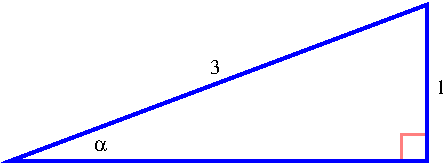
\includegraphics[width=1\linewidth]{finding-angles-ex-1}
\end{image}

\begin{explanation}
Because we know the hypotenuse and the side opposite $\alpha$, we observe that $\sin(\alpha) = \frac{1}{3}$.  Rewriting this statement using inverse function notation, we have equivalently that $\alpha = \arcsin\!\bigg(\frac{1}{3}\bigg)$, which is the exact value of $\alpha$.  Since this is not one of the known special angles on the unit circle, we leave it in this form.%
\par
%
We can now find the remaining leg's length and the remaining angle's measure.  If we let $x$ represent the length of the horizontal leg, by the Pythagorean Theorem we know that
%
\begin{equation*}
x^2 + 1^2 = 3^2\text{,}
\end{equation*}
and thus $x^2 = 8$ so $x = \sqrt{8}$.  Calling the remaining angle $\beta$, since $\alpha + \beta = \frac{\pi}{2}$, it follows that
%
\begin{equation*}
\beta = \frac{\pi}{2} - \arcsin\!\bigg(\frac{1}{3}\bigg) \text{.}
\end{equation*}

\end{explanation}
\end{example}

\begin{example}

Let's consider the composite function $h(x) = \cos(\arcsin(x))$.  \\
Does it makes sense to consider this function? Let's think $\dots$ \\
This function makes sense to consider since the arcsine function has range $[-1,1]$, on which we may evaluate the cosine function. In the questions that follow, we investigate how to express $h$ without using trigonometric functions at all.%
\par
%
\begin{enumerate}

\item What is the domain of $h$?  The range of $h$? \\
%
\begin{explanation}
The domain of $h$ is the domain of the inner function, $\arcsin(x)$, which produces values within the domain of the outer function, $\cos(z)$. As noted at the beginning, since the range of $\arcsin(x)$ is $[-1,-1]$ contained in $(-\infty,\infty)$, the domain of $\cos(z)$, the domain of $h$ is simply the domain of $\arcsin(x)$. \\
The domain of $h$ is therefore $[-1,1]$.

Now, the range of $h$ will be the output of the outer function when the input is the range of the inner function. In other words, we are looking for the values that $\cos(z)$ attains on the interval $[-1,1]$. Since cosine is symmetric about the $y$-axis, this is the same as the values attained by $\cos(z)$ on the interval $[0,1]$. Thus, we have a range of $[\cos(1),1]$.
\end{explanation}
%
\item Since the arcsine function produces a value we can consider as an angle, let's say that $\theta = \arcsin(x)$,  so that $\theta$ is the angle whose sine is $x$.  By definition, we can picture $\theta$ as an angle in a right triangle with hypotenuse $1$ and a vertical leg of length $x$, as shown in the image on the left below.  Use the Pythagorean Theorem to determine the length of the horizontal leg as a function of $x$. \\
%
\begin{explanation}
First we recall the Pythagorean Theorem, $a^2 +b^2 = c^2$, where $c$ is the hypotenuse of a right triangle with legs of lengths $a,b$. Hence, in this instance, let's denote the length of the horizontal leg by $y$, so we have $y^2 + x^2 = 1^2$. In other words
%
$$y = \sqrt{1-x^2},$$
%
since a triangle leg will have positive length.
\end{explanation}
%
\begin{image}
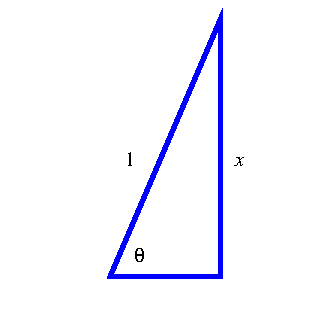
\includegraphics{inv-trig-cosarcsin.pdf}
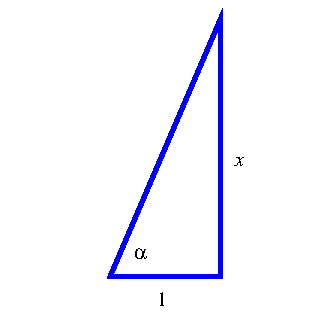
\includegraphics{inv-trig-cosarctan.pdf}
\end{image}%


The right triangle on the left corresponds to the angle $\theta = \arcsin(x)$.
%
The right triangle on the right corresponds to the angle $\alpha = \arctan(x)$.
%
\item What is the value of $\cos(\theta)$ as a function of $x$?  What have we shown about $h(x) = \cos(\arcsin(x))$?\\
%
\begin{explanation}
Here, we use the results of part (b). Since we know that $\cos(\theta)$ is $\frac{adj}{hyp}$ and $\theta = \arcsin(x)$,
%
$$\cos(\theta) = \frac{y}{1} = \sqrt{1-x^2}.$$
From this we see that
%
$$h(x) = \cos(\arcsin(x)) = \sqrt{1-x^2}.$$
\end{explanation}

%
\item How about the function $p(x) = \cos(\arctan(x))$?  How can you reason similarly to write $p$ in a way that doesn't involve any trigonometric functions at all?  (Hint:  let $\alpha = \arctan(x)$ and consider the right triangle on the right above.)\\
%
\begin{explanation}
We can now use a similar approach to determine $p$ as an algebraic function of $x$. Let $\alpha = \arctan(x)$, so that $p(x)= \cos(\arctan(x)) = \cos(\alpha)$.

In the second triangle we must find the value of the hypotenuse, call it $y$. Then
$$y^2 = 1^2 + x^2 \text{ which implies } y = \sqrt{1+x^2}.$$
%
Now, $\cos(\alpha) = \frac{1}{y} = \frac{1}{\sqrt{1+x^2}}$. Therefore, 
%
$$p(x) = \cos(\arctan(x)) = \frac{1}{\sqrt{1+x^2}}.$$
\end{explanation}
%
\end{enumerate}

\end{example}

\section{Using Inverse Trig in Applied Contexts}
%
Now that we have developed the (restricted) sine, cosine, tangent, and secant functions and their respective inverses, in any setting in which we have a right triangle together with one side length and any one additional piece of information (another side length or a non-right angle measurement), we can determine all of the remaining pieces of the triangle. In the example that follows and the homework, we explore these possibilities in a variety of different applied contexts.
%
\begin{example}%
A roof is being built with a ``7-12 pitch.'' This means that the roof rises $7$ inches vertically for every $12$ inches of horizontal span; in other words, the slope of the roof is $\frac{7}{12}$. 
%
\begin{enumerate}
\item What is the exact measure of the angle the roof makes with the horizontal? \\
\begin{explanation}
Looking at a side view of the house, we may divide the triangle of the roof in half to get a right triangle with legs 7 and 12 feet long. We want to find the angle of inclination ($\theta$ in the diagram below), which satisfies the equation $\tan(\theta) = \frac{7}{12}$. In other words, we wish to find $\theta = \arctan\!\Big(\frac{7}{12}\Big)$. As in Example 1, this does not match one of our known values, so we leave it in this form since this is the {\em exact} value.

\end{explanation}

\begin{image}%[Roof Side-view]
		  \begin{tikzpicture}
		    \coordinate (C) at (0,2);
		    \coordinate (D) at (4,2);
		    \coordinate (E) at (4,4.5);
		    \coordinate (F) at (8,2);
		    %\tkzMarkRightAngle(C,D,E)
		    %\tkzMarkAngle(C,E,D)
		   % \draw[decoration={brace,mirror,raise=.2cm},decorate,thin] (0,2)--(4,2);
		   % \draw[decoration={brace,mirror,raise=.2cm},decorate,thin] (4,2)--(4,6.5);
		  %  \draw[decoration={brace,raise=.2cm},decorate,thin] (0,2)--(4,6.5);
		    \draw[very thick] (D)--(E)--(C)--cycle;
		    \draw[very thick] (D)--(E)--(F)--cycle;
		   \node at (4.2,3) {7};
		   \node at (2.5,2.2) {12};
		   % \node[rotate=48.5] at (1.4-.1,3.8+.6) {C};
		    \node at (.6,2.2) {$\theta$};
		     \node at (3.7,4) {$\alpha$};
		  \end{tikzpicture}
		\end{image}
	The image above is a side-view of the roof.

\item What is the exact measure of the angle at the peak of the roof (made by the front and back portions of the roof that meet to form the ridge)?\\
%
\begin{explanation}
This will be double the angle at the top of the right triangle we used for part (a), since we had bisected this angle to form the right triangle. We now wish to find the angle $\alpha$ satisfying $\tan(\alpha) = \frac{12}{7}$. In other words, we are looking for $\alpha = \arctan\!\Big(\frac{12}{7}\Big)$. Once again, this is not a common angle, so it is the {\em exact} value. We need double this angle, so $2\alpha = 2\arctan\!\Big(\frac{12}{7}\Big)$ is our solution.
\end{explanation}
\end{enumerate}
\end{example}

\begin{exploration}
On a baseball diamond (which is a square with $90$-foot sides), the third baseman fields the ball right on the line from third base to home plate and $10$ feet away from third base (towards home plate).  
Give exact solutions without using a computational device.%
%
\begin{enumerate}
\item When he throws the ball to first base, what angle does the line the ball travels make with the first base line?
%
\item What angle does it make with the third base line? Draw a well-labeled diagram.
%
\item What angles arise if he throws the ball to second base instead?
%
\end{enumerate}
\end{exploration}

\begin{exploration}
Give exact solutions without using a computational device.
%
A camera is tracking the launch of a SpaceX rocket. The camera is located $4000$' from the rocket's launching pad, and the camera elevates in order to keep the rocket in focus. 
\begin{enumerate}
\item At what angle is the camera tilted when the rocket is $3000$' off the ground?
%
\item[] Now, rather than considering the rocket at a fixed height of $3000$ ft, let its height vary and call the rocket's height $h$. 

\item Determine the camera's angle, $\theta$ as a function of $h$, and compute the average rate of change of $\theta$ on the intervals $[3000,3500]$, $[5000,5500]$, and $[7000,7500]$. 
%
\item What do you observe about how the camera angle is changing?
%
\end{enumerate}
\end{exploration}


%\typeout{************************************************}
%\typeout{section}
%\typeout{************************************************}



\section{Further Exploration}

When composing trigonometric functions with inverse trigonometric functions, the expressions can often be rewritten as algebraic expressions of $x$. We will see two examples of this below.

\begin{example}
Rewrite the following values as algebraic expressions of $x$ and give the domain on which these equivalences are valid.
\begin{enumerate}
\item $\cos(\arctan(x))$.\\
%
\begin{explanation}
Recall that we found this expression in Example 2, part (d), to be
$$\cos(\arctan(x)) = \frac{1}{\sqrt{1+x^2}}.$$ %  for all $x$  \\
%
Now, we must find the domain for which this is true.

We start by checking the domain of the outer function, $\cos(y)$. Since the domain of the cosine function is all real numbers, we do not have any restrictions to consider here. Thus, our only concern is the domain of the arctangent function, which is also the real line. Thus, we see that 
$$\cos(\arctan(x)) = \frac{1}{\sqrt{1+x^2}} \text{ for all } x \text{ in } (-\infty, \infty).$$  
%To see this, we start by simplifying $\cos(\arctan(x))$ by letting $t = \arctan(x)$, so that $\tan(t) = x$ for $t$ in the domain of restricted tangent, $(-\pi/2,\pi/2)$. We now need a formula for $\cos(t)$, which is defined for all $t$ in this domain.
%Use $1 + \tan^2(t) = \sec^2(t) = \frac{1}{\cos^2(t)}$
\end{explanation}
%
\item $\sin(\arccos(2x))$. \\
%
\begin{explanation}
$\sin(\arccos(2x)) = \sqrt{1-4x^2}$ given $x$ in $\Big[-\!\frac{1}{2}, \frac{1}{2}\Big]$\\
%
Again, to see this, we begin by setting $t = \arccos(2x)$, so that $\cos(t) = 2x$ for $t$ in the domain of restricted cosine, $[0,\pi]$. In other words, we have $\cos(t) = 2x$ for $t$ in $[0, \pi]$, and must find a formula for $\sin(t)$. Now, we must relate sine and cosine, for which we use the well-known trigonometric identity $\sin^2(t) + \cos^2(t) = 1$. Re-writing this to solve our equation, we see that we have $\sin^2(t) + (2x)^2 =1$, which is equivalent to 
%
$$\sin(t) = \pm \sqrt{1-4x^2}.$$
%
Since sine is positive on the interval $[0,\pi]$, where we defined $t$, we choose the positive square root, and observe that $\sin(\arccos(2x)) = \sqrt{1-4x^2}$, as desired.

Finally, to establish the domain on which this equivalence holds, we
recall that the domain of arccosine is $[-1,1]$. Since we consider $\arccos(2x)$, we want $2x$ in $[-1,1]$. This is equivalent to $x$ in $\Big[-\frac{1}{2}, \frac{1}{2} \Big]$, and so our work is done.
\end{explanation}
%
\end{enumerate}
\end{example}


\subsection{A Note on Triangles}
We can now use trigonometry to find angles of right triangles if we know the side lengths and side lengths of right triangles if we know the angles.  You might be wondering, ``What about triangles that are not right triangles? Can we use trig to learn anything about those?''  It turns out that the Law of Sines and the Law of Cosines gives use a way to analyze other triangles beyond just right triangles using trig functions.  For more information about this topic, see \link[Laws of Sines and Cosines by Katherine Yoshiwara]{https://yoshiwarabooks.org/trig/chap3.html}.


\begin{summary}
Anytime we know two side lengths in a right triangle, we can use one of the inverse trigonometric functions to determine the measure of one of the non-right angles.  For instance, if we know the values of $\text{opp}$ and $\text{adj}$ in the triangle pictured below, then since%
\begin{equation*}
\tan(\theta) = \frac{\text{opp}}{\text{adj}}\text{,}
\end{equation*}
it follows that $\theta = \arctan\!\bigg(\frac{\text{opp}}{\text{adj}}\bigg)$.%
%
\begin{image}
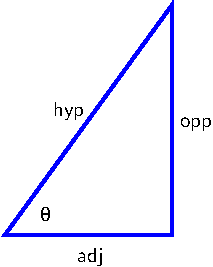
\includegraphics[width=.5\linewidth]{right-triangle-SOH-CAH-TOA.pdf}
\end{image}
%
\par
%
If we instead know the hypotenuse and one of the two legs, we can use either the arcsine or arccosine function accordingly.%

Similarly, we may use this relationship along with the Pythagorean Theorem to find algebraic expressions for compositions of trig functions with trig inverses (see Example 2). The trig identities we learned in Section 10 are also useful to rewrite the compositions of functions as algebraic expressions (see Example 4). 
%
%For situations other than angles or ratios that involve the $16$ special points on the unit circle, technology is required in order to evaluate inverse trignometric functions.  For instance, from the unit circle we know that $\arccos(\frac{1}{2}) = \frac{2\pi}{3}$ (exactly), but if we want to know $\arccos(\frac{1}{3})$, we have to estimate this value using a computational device such as \emph{Desmos}.  We note that ``$\arccos(\frac{1}{3})$'' is the exact value of the angle whose cosine is $1/3$.%

\end{summary}

\end{document}
